% !TEX TS-program = pdflatex
% !TEX encoding = UTF-8 Unicode

\documentclass[14pt,a4paper]{extarticle}
%\usepackage{etex}
\usepackage{Diplo}
\usepackage{extsizes}
\usepackage{cmap}
\usepackage[utf8]{inputenc}	
\usepackage[T2A]{fontenc}
\usepackage{graphicx,epsfig}
\usepackage[english,russian]{babel}
\usepackage{geometry}
\geometry{left=3cm}
\geometry{right=2cm}
\geometry{top=2cm}
\geometry{bottom=2cm}
\bibliographystyle{abbrv}
\usepackage[nottoc,numbib]{tocbibind}
\usepackage{hyperref}
\usepackage{babelbib}
\usepackage[section]{placeins}
\usepackage[hypcap,labelfont=bf,justification=centering]{caption}
\usepackage{titlesec}
\newcommand{\sectionbreak}{\clearpage}

\usepackage{subcaption}
\DeclareCaptionLabelFormat{gostfigure}{Рисунок #2}
\captionsetup[figure]{labelformat=gostfigure}
\DeclareCaptionLabelSeparator{gost}{.~}
\captionsetup{labelsep=gost}


\hyphenpenalty=9999
%\sloppy
\emergencystretch=3em
\tolerance=9999

\usepackage{amsfonts,mathtext,cite,float}

\newtheorem{experiment}{Эксперимент}

%\usepackage{setspace}
%\onehalfspace
\linespread{1.5} % полуторный интервал
%\renewcommand{\rmdefault}{ftm} % Times New Roman
\frenchspacing

\usepackage{minted}


\begin{document}
{
\fontsize{12pt}{15pt}
\thispagestyle{empty}
\begin{center}
    \sc
        Министерство образования и науки Российской Федерации\\
        Московский физико-технический институт
        {\rm(государственный университет)}\\
        Факультет инноваций и высоких технологий\\
        Кафедра <<Анализ данных>>\\[35mm]
    \rm\large
        Вольхин Артем Васильевич\\[10mm]
    \bf\Large
	    Влияние микротрубочек на скорость образования стрессовых гранул\\[10mm]
    \rm\normalsize
        010400 --- Прикладная математика и информатика\\[10mm]
    \sc
        Выпускная квалификационная работа бакалавра\\[10mm]
\end{center}
\hfill\parbox{80mm}{
    \begin{flushleft}
    \bf
        Научный руководитель:\\
    \rm
        Шпильман Алексей Александрович\\[5cm]
    \end{flushleft}
}
\vfill
\begin{center}
    Москва\\
    2013
\end{center}
}


\clearpage
\tableofcontents
\clearpage


\section{Введение} % 1-2 страницы
	 Стрессовые гранулы - скопления РНП в цитоплазме живых клеток, наблюдающиеся после воздействия стрессовых факторов, например, теплового шока, окислительного стресса, ультрафиолетового облучения. В живых клетках образование стрессовых гранул занимает порядка 10-20 минут. Размеры стрессовых гранул составляют обычно от 20 нм до нескольких мкм. Столь быстрое образование нарушает законы затрудненной диффузии, согласно которым большие гранулы практически неподвижны.

	 Роль микротрубочек в образовании стрессовых гранул до сих пор не до конца изучена. Существует предположение, что без микротрубочек образование стрессовых гранул невозможно, однако существуют и другие предположения. В частности, что микротрубочки ускоряют образование стрессовых гранул. Одним из механизмов может быть осуществление транспорта компонентов стрессовых гранул микротрубочками, облегчающий их встречу в пространстве клетки. Для доказательства этого механизма необходимо количественное изучение динамики сборки стрессовых гранул в присутствии и отсутствии микротрубочек в клетке и компьютерное моделирование такой системы.
	 
	 Изучение числа, расположения и движения стрессовых гранул при различных условиях, а также взаимодействия со структурой микротрубочек в клетке, является основной задачей исследования стрессовых гранул. Важным для понимания динамики стрессовых гранул является определение их скорости, типа движения и взаимодействия гранул между собой.
	 
	 Целью данной работы является построение модели движения и взаимодействия стрессовых гранул между собой и с микротрубочками и проверка на этой модели достоверности имеющихся теоретических формул. Выбор численного моделирования вместо изучения живых клеток с помощью флуоресцентной микроскопии обусловлен тем, что разрешающая способность микроскопа позволяет наблюдать за частица размером не менее 100 нм, в то время как радиусы стрессовых гранул могут быть от 20 нм. Модель представляет собой частицы, случайным образом перемещающиеся в некотором объеме, и сеть микротрубочек, вдоль которых они могут скользить.



\section{Обзор литературы} % 15-20 страниц

 \subsection{Броуновское движение}
	 Броуновское движение~--- беспорядочное движение микроскопических видимых, взвешенных в жидкости или газе частиц твердого вещества, вызываемое тепловым движением частиц жидкости или газа. Броуновское движение никогда не прекращается. Броуновское движение связано с тепловым движением, но не следует смешивать эти понятия. Броуновское движение является следствием и свидетельством существования теплового движения.
	 
	 Броуновское движение~--- наиболее наглядное экспериментальное подтверждение представлений молекулярно-кинетической теории о хаотическом тепловом движении атомов и молекул. Если промежуток наблюдения достаточно велик, чтобы силы, действующие на частицу со стороны молекул среды, много раз меняли своё направление, то средний квадрат проекции её смещения на какую-либо ось (в отсутствие других внешних сил) пропорционален времени.
	 
	 Количественное описание броуновского движения было предложено Альбертом Эйнштейном в 1905 г. Его теория содержит 2 основные части. Первая часть "--- формулировка уравнения диффузии "--- описывает связь коэффициента диффузии и среднеквадратичного смещения (mean squared displacement, MSD) броуновской частицы в одномерном случае: 
\begin{equation}
\overline{x^2} = 2Dt
\end{equation}
(для двумерного случая: $\overline{r^2} = 4Dt$, где $r^2 = x^2 + y^2$). Вторая "--- связывает коэффициент диффузии с измеряемыми физическими величинами~\cite{Einstein:1905ys}:
\begin{equation}
D = \frac{RT}{N} = \frac{1}{6\pi kP}.
\end{equation}

	Теория Эйнштейна была проверена и подтверждена опытами Жана Батиста Перрена в 1908--1909 гг. Справедливость формул была доказана для частиц с размерами от 0,212 мкм до 5,5 мкм~\cite{Perrin:1906ys}.



\subsection{Стрессовые гранулы}
\begin{figure}[hbt]\centering
\includegraphics[width=0.9\columnwidth]{../pics/stressgranules.jpg}
\caption{Внешний вид стрессовых гранул при флуоресцентной микроскопии.}
\label{fig:sg-content}
\end{figure}
	 Стрессовые гранулы - скопления РНП в цитоплазме живых клеток, наблюдающиеся после воздействия стрессовых факторов, например, теплового шока, окислительного стресса, ультрафиолетового облучения \cite{Kedersha27121999}. После прекращения стрессирующего воздействия стрессовая гранула рассасывается. В состав стрессовых входят мРНК, РНК-связывающие белки, которые могут под действием факторов инициации трансляции elF1, elF3, elF4 использоваться для хранения, сортировки или других неизвестных процессов \cite{Anderson:2008ys, Ivanov:2006ul}. Для включения в состав стрессовой гранул мРНА не должна обладать никакой особой структурой, а вот не входящие в ее состав содержат в себе специальную последовательность сигналов, например Hsp70 \cite{Kedersha:2002kx}. Предполагается, что образование стрессовых гранул является следствием ингибирования трансляции на стадии инициации, в частности, за счет фосфорилирования elF2a \cite{Kedersha:2002vn}. В результате этого фосфорилирования в клетке резко снижается количество тройственного комплекса, и на 5’ концах мРНК собирается неканонический инициаторный комплекс, не содержащий тройственного комплекса. Получающиеся мРНП-частицы объединяются в цитоплазме в стрессовые гранулы.
	 
\begin{figure}[hbt]\centering
\includegraphics[width=0.9\columnwidth]{../pics/Sg-content.png}
\caption{Образование стрессовой гранулы.}
\label{fig:sg-content}
\end{figure}

	 Для минимизации ущерба мРНК, образование стрессовых гранул должны происходить достаточно быстро. В живых клетках оно занимает порядка 10-20 минут. Размеры стрессовых гранул составляют обычно от 20 нм до нескольких мкм. Однако, столь быстрое образование нарушает законы затрудненной диффузии, согласно которым большие гранулы практически неподвижны.
	 
	 Стрессовые гранулы являются достаточно плотными структурами. Несмотря на достаточно продолжительную историю их исследования, попытки выделить их in vitro оказались неудачными. Стрессовые гранулы изучают в основном методами световой микроскопии, используя иммунофлуоресцентное окрашивание, экспрессию в клетках белков-маркеров стрессовых гранул, слитых с флуоресцентными белками, гибридизацию с ДНК-зондами. Изучение числа, расположения в клетке и движения стрессовых гранул при различных стрессовых условиях, а также взаимодействие со структурой микротрубочек в клетке, является основной задачей исследования стрессовых гранул.
	 
	 Роль микротрубочек в образовании стрессовых гранул до сих пор не до конца изучена. Существует предположение, что без микротрубочек образование стрессовых гранул не возможно, однако это кажется не верным. Более верным кажется предположение, что микротрубочки ускоряют образование стрессовых гранул. Каким образом также не совсем ясно, считается, что микротрубочки осуществляют транспорт компонентов стрессовых гранул, облегчающий их встречу в пространстве клетки. Для доказательства этого механизма необходимо количественное изучение динамики сборки стрессовых гранул в присутствии и отсутствии микротрубочек в клетке. Существенным при это является вопрос, достоверна ли оценка интенсивности образования стрессовых гранул по доле клеток, в которых они образовались.


 \subsection{Микротрубочки}
 Микротрубочки~--- это белковые внутриклеточные структуры, входящие в состав цитоскелета. Микротрубочки представляют собой полые внутри цилиндры диаметром 25 нм. Длина их может быть от нескольких микрометров до, вероятно, нескольких миллиметров в аксонах нервных клеток. Их стенка образована димерами тубулина. Микротрубочки, подобно актиновым микрофиламентам, полярны: на одном конце происходит самосборка микротрубочки, на другом — разборка. В клетках микротрубочки играют роль структурных компонентов и участвуют во многих клеточных процессах, включая митоз, цитокинез и везикулярный транспорт.
 
 Микротрубочки~--- это структуры, в которых 13 протофиламентов, состоящих из гетеродимеров $\alpha$- и $\beta$- тубулина, уложены по окружности полого цилиндра. 
 Внешний диаметр цилиндра около 25 нм, внутренний~--- около 15.
Один из концов микротрубочки, называемый плюс-концом, постоянно присоединяет к себе свободный тубулин. От противоположного конца (минус-конца) тубулиновые единицы отщепляются.
В образовании микротрубочки выделяют три фазы:

\begin{itemize}
\item замедленная фаза, или нуклеация. Это этап зарождения микротрубочки, когда молекулы тубулина начинают соединяться в более крупные образования. Такое соединение происходит медленнее, чем присоединение тубулина к уже собранной микротрубочке, поэтому фаза и называется замедленной;
\item фаза полимеризации, или элонгация. Если концентрация свободного тубулина высока, его полимеризация происходит быстрее, чем деполимеризация на минус-конце, за счет чего микротрубочка удлиняется. По мере её роста концентрация тубулина падает до критической и скорость роста замедляется вплоть до вступления в следующую фазу;
\item фаза стабильного состояния. Деполимеризация уравновешивает полимеризацию, и рост микротрубочки останавливается.
\end{itemize}

	Лабораторные исследования показывают, что сборка микротрубочек из тубулинов происходит только в присутствии гуанозинтрифосфата и ионов магния.

	Микротрубочки в клетке используются в качестве «рельсов» для транспортировки частиц. По их поверхности могут перемещаться мембранные пузырьки и митохондрии. Транспортировку по микротрубочкам осуществляют белки, называемые моторными. Это высокомолекулярные соединения, состоящие из двух тяжёлых (массой около 300 кДа) и нескольких лёгких цепей. В тяжёлых цепях выделяют головной и хвостовой домены. Два головных домена связываются с микротрубочками и являются собственно двигателями, а хвостовые — связываются с органеллами и другими внутриклеточными образованиями, подлежащими транспортировке.
Выделяют два вида моторных белков:

\begin{itemize}
\item цитоплазматические динеины
\item кинезины
\end{itemize}

	Динеины перемещают груз только от плюс-конца к минус-концу микротрубочки, то есть из периферийных областей клетки к центросоме. Кинезины, напротив, перемещаются к плюс-концу, то есть к клеточной периферии.
Перемещение осуществляется за счёт энергии АТФ. Головные домены моторных белков для этого содержат АТФ-связывающие участки.
Помимо транспортной функции, микротрубочки формируют центральную структуру ресничек и жгутиков — аксонему. Типичная аксонема содержит 9 пар объединённых микротрубочек по периферии и две полных микротрубочки в центре. Из микротрубочек состоят также центриоли и веретено деления, обеспечивающее расхождение хромосом к полюсам клетки при митозе и мейозе. Микротрубочки участвуют в поддержании формы клетки и расположения органоидов (в частности, аппарата Гольджи) в цитоплазме клеток.

 
\subsection{Материалы}
	В большинстве работ исследование микротрубочек проводится при помощи световой микроскопии, используя иммунофлуоресцентное окрашивание \cite{Nadezhdina:2010uq}.
Исследования проводили на клетках HeLa (человеческая карцинома шейки матки), CV-1 (эпителий почки зеленой мартышки) и CHO (яичник китайского хомяка). Клетки выращивали на среде, содержащей 45\% среды F12, 45\% среды DMEM, 10\% эмбриональной сыворотки крупного рогатого скота  c добавлением гентамицина на пластиковой культуральной посуде при стандартных условиях (температура $37^{\circ}~\mathrm{C}$, содержание углекислого газа в среде –5\%). Для экспериментов культивируемые клетки рассаживали на покровные стекла.

	Для разборки клеточных микротрубочек в среду добавляли нокодазол до конечной концентрации 6 мкг/мл на 2 ч. Для индукции СГ использовали арсенит натрия ($NaH_2AsO_3$); максимальная конечная концентрация арсенита в среде культивирования составляла 250 мкМ (для клеток HeLa) и 625 мкМ (для клеток CV-1). Время воздействия арсенитом составляло 30--60 мин. Для расщепления стрессовых гранул использовали циклогексамид (CHX), а для разборки микрофилламентов~--- летрункулин.

	Клетки фиксировали в охлажденном до $-20^{\circ}~\mathrm{C}$ абсолютном метаноле. Для иммунофлуоресцентного окрашивания покровные стекла с клетками инкубировали в течение 30 мин с первыми антителами, разведенными на PBS, промывали два раза по 5--7 мин PBS и инкубировали в течение 30 мин со вторыми антителами, конъюгированными с флуорохромами. После инкубации со вторыми антителами стекла промывали три раза по 5--7 мин буфером PBS и заключали в Aqua Poly/Mount (Polysciences, США).

	В работе использовали поликлональные кроличьи антитела к eIF3а (Шанина и др., 2001) и моноклональные антитела к тубулину DM-1A (Sigma, США), антитела против IgG кролика и IgG мыши, конъюгированные с тетраметилродаминизотиоцианатом (TRITC) или с флуоресцеинизотиоцианатом (FITC) (Molecular Probes, США).

	Препараты клеток просматривали в микроскопе Axiovert-200М (Carl Zeiss, Германия) с объективами Planapo 63х и 100х. Фотографии (16-битовые черно- белые изображения) получали с помощью цифровой видеокамеры AxioCam HRc, управляемой программным обеспечением AxioVision 3.1 (Carl Zeiss Vision, Германия).


\subsection{Сбор и анализ данных}
	Серии изображений сохранялись в виде 16-битных цифровых файлов и обрабатывались в приложении MetaMorph (Universal imaging). Стрессовые гранулы отслеживались при помощи Point-Tracking функции в MetaMorph. Данные импортировались в Excel для вычисления мгновенной скорости. Разработанная авторами программа вычисляла и рисовала график зависимости среднеквадратичного отклонения $MSD$ от времени $\tau$, согласно \cite{Saxton:1993uq}.
MSD вычислялось для каждой частицы в каждый момент времени как
$$
MSD(n \tau) = \frac{1}{N - n} \sum_{i=1}^{N - n}
[(x((i+n)\tau) - x(i\tau))^2 + (y((i+n)\tau) - y(i\tau))^2]
$$

На основе полученной зависимости вычислялся коэффициент диффузии
$$
D_{app} = MSD(n\tau) / \Delta \tau
$$
согласно \cite{Heinzer:2008fk}.

	Для выделения стрессовых гранул и определения посещенной области видео-кадры сперва нормализовались при помощи Bleaching Normalization плагина из ImageJ. Число стрессовых гранул и общая посещенная площадь вычислялись через Region Measurments и Integrated Morphometry из Metamorph и ImageJ Analyze Particles plug-in.

	Временные серии FRAP анализировались в MetaMorph. Сырые данные флуоресцентной интенсивности сперва регулировались путем вычитания фона в каждый момент времени. Интенсивность каждой восстановленной гранулы нормализовалась к среднему уровню сигнала и по этим данным строились графики в Origin software (OriginalLab Corp.).

\begin{figure}[htb]\centering
\includegraphics[width=\columnwidth]{../pics/0.jpg}
\caption{Движение, объединение и расщепление стрессовых гранул.}
%\label{fig:velocity}
\end{figure}


\subsection{Движение, объединение и разъединение СГ}
	 Было выяснено, что стрессовые гранулы в цитоплазме движутся, объединяются в большие гранулы и, наоброт, разъединяются. В течение первых 5--7 минут эксперимента число стрессовых гранул росло, после чего начало снижаться. После 10--12 минут их число стало постоянным. Уменьшение числа стрессовых гранул объясняется их объединением и формированием больших гранул. Двигаться гранулы начали с момента образования и продолжали даже через 150 минут после начала эксперимента. Существенной зависимости от температурной обработки клеток выявлено не было. Многие гранулы хаотически двигались в цитоплазме, некоторые были практически неподвижны, в то время как другие преодолевали достаточно большие расстояния за короткие промежутки времени \cite{Sheetz:1999uq}.
	 
	 Объединение гранул происходило при их столкновении: две гранулы сливались в одну и продолжали движение уже как одна гранула. Расщепление происходило только при добавлении CHX следующим образом: гранула разделялась на части, которые разлетались; выглядело так, будто часть гранулы выдергивает какая-то внешняя сила. Без добавления CHX расщепления гранул не наблюдалось.
	 
	 Для исключения связи наблюдаемых результатов с типом клеток (использовались клетки HeLa), были также проведены эксперименты с клетками CV-1 и CHO. Предполагается, что подвижность стрессовых гранул~--- это непосредственно их свойство, а не влияние определенного типа клеток.


\subsection{Движение СГ за счет диффузии}
	Была исследована природа подвижности стрессовых гранул. Во-первых, была измерена мгновенная скорость (на 2--3 секундных интервалах). Рассматривались 12 клеток, 75 стрессовых гранул на 6524 временных интервалах. Около 10\% гранул были неподвижны, у 8\% скорость была меньше $0.2~\textup{мкм/с}$, максимальная скорость была порядка $0.7~\textup{мкм/с}$, а средняя (не учитывая неподвижные гранулы)~--- $0.1~\textup{мкм/с}$
(\autoref{fig:velocity}). Не было выявлено существенной зависимости скорости гранул от их размера. Изучив траектории движения за 3 минуты, можно найти среди них признаки ограниченной, затрудненной и обычной диффузии, а также направленного движения \cite{Saxton:1995kx}. Среди наблюдаемых гранул 10\% двигались направленно, 17\%~--- согласно обычной диффузии, а 73\%~--- затрудненной диффузии.
	
\begin{figure}[htb]\centering
\includegraphics[width=0.8\columnwidth]{../pics/2.jpg}
\caption{Распределение скоростей.}
\label{fig:velocity}
\end{figure}

	Посчитав MSD и $D_{app}$ получили, что коэффициент диффузии со временем уменьшается, сходясь к ассимптотическому значению
$1.9~\times~10^{-3}~\textup{мкм}^2\textup{/с}$. Исследовав посещенную гранулами область получили, что за 4 минуты движения она в 3 раза превышает суммарный размер самих гранул. Предположительно, стрессовый гранулы способны собирать все подходящие компоненты с посещенной территории, такие как другие мелкие стрессовые гранулы.
	

\subsection{Движение СГ вдоль микротрубочек}
	Плотная и хаотическая система микротрубочек в клетках HeLa не позволяет отслеживать движение стрессовых гранул вдоль микротрубочек. Для экспериментов были взяты клетки CHO с радиальной системой микротрубочек и наблюдали при помощи флюоресцентной микроскопии за живыми клетками. Наблюдения подтвердили движение стрессовых гранул вдоль микротрубочек и формирование скоплений. Их движение было непостоянным: гранулы двигались, останавливались, продолжали движение в обратном направлении. Но при этом не отрывались от микротрубочек. Типичные размеры гранул составляли от 200 нм до 5 мкм.
	
	При добавлении нокодазола для разрушения микротрубочек стрессовые гранулы не пропадали, более того, их количество увеличивалось. Из чего можно сделать вывод, что микротрубочки не являются необходимыми для образования стрессовых гранул. Отличием стало лишь то, что концетрация гранул стала более беспорядочная по всему объему цитоплазмы, исчезли сгустки.


\subsection{Роль микротрубочек в движении СГ}

\begin{figure}[htb]\centering
\includegraphics[width=0.9\columnwidth]{../pics/3.jpg}
\caption{Анализ диффузионного движения. d.m. — directed motion; s.d. — simple diffusion; o.d. — obstructed diffusion; c.d. — confined diffusion.}
\label{fig:diffusive}
\end{figure}

После разрушения микротрубочек нокодазолом подвижность стрессовых гранул значительно снизилась. Так, только у 1.5\% гранул скорость осталась более $0.2~\textup{мкм/с}$ (\autoref{fig:diffusive}), а средняя скорость упала до $0.076~\textup{мкм/с}$. Движение уже 92\% гранул стало напоминать затрудненную диффузию, тогда как доля гранул с ограниченной и обычной диффузией снизилась до 3\% и 5\% соответственно. Гранул с направленным движением не осталось вовсе. Коэффициент диффузии уменьшился более чем в три раз и стал равен $6~\times~10^{-4}~\textup{мкм}^2\textup{/с}$.

	Для изучения роли микротрубочек в движении стрессовых гранул микротрубочки были зафиксированы при помощи таксола. Скорость стрессовых гранул уменьшилась всего на 6\%, из чего следует, что не самостоятельное движение микротрубочек увеличивало скорость стрессовых гранул, а сам факт наличия микротрубочек. Это легко объяснить, если считать, что стрессовые гранулы находят микротрубочку, прикрепляются к ней и дальше двигаются вдоль нее.

	Проведя аналогичные эксперименты со стрессовыми гранулами и микрофиламентами, выяснилось, движение СГ слабо зависит от наличия или отсутствия микрофиламентов. Таким образом, именно микротрубочки играют ключевую роль в транспорте стрессовых гранул.
	
	В других работах \cite{Chernov:2009fk} утверждается, что движение миктротрубочек существенно влияет на подвижность стрессовых гранул. Согласно их наблюдениям, микрофилламенты припятствуют движению достаточно больших стрессовых гранул (типичное расстояние между микрофилламентами - 100 нм). В результате стрессовые большие гранулы остаются неподвижны и могут продолжать увеличиваться в размерах за счет слияния с более мелкими, столкнувшимися с ними. Однако движение микротрубочек позволяет перемещать большие гранулы, застрявшие в сети микрофилламентов~--- при элонгации гранулы, находящиеся вблизи минус-конца <<тянутся>> за микротрубочкой. При этом предположение о движении стрессовых гранул вдоль микротрубочек не опровергается, но высказываются сомнения в эффективности такого метода движения.



\subsection{Теоретические оценки}
	Для изучения модели движения стрессовых гранул интересным представляется таких величин, как среднее время столкновения между гранулами, время до столкновения стрессовой гранулы с микротрубочкой, время до столкновения между стрессовыми гранулами на одной микротрубочки и другие. работе \cite{Chernov:2009fk} представлены теоретические оценки для этих величин.

	Так, время $t_g$, требуемое для формирования стрессовой гранулы радиуса $R$ равно
\begin{equation} \label{eq:tg}
	t_g = t_d \cdot (R/r)^{df},
\end{equation}

где $t_d \approx \eta / (K_B T C_{RNP}) \approx 1 / (4 \pi D r C_{RNP})$~--- время между столкновениями mRPN, $\eta$~--- вязскость цитоплазмы, $r$ и $C_{RNP}$~--- радиус и концетрация изначальных mRNP частиц, соответственно, $D$~--- коэффициент диффузии, $K_B T$~--- тепловая энергия, а $df$~--- фрактальная размерность, равная $\sim1.8$ \cite{Weitz:1986pd}. В клетке цитоплазмы млекопитающих содержится  $\sim$ 15,000--150,000 мРНА молекул, объем клетки порядка 2000 мкм$^3$, а значит концетрация мРНА 12--120 нМ. $r \simeq 10$ нм, $\eta \simeq 10^{-2}~pascal/s$, $T~=~37^{\circ}~C$.
При этих параметрах $t_d \sim 0.2s$, то есть для формирования стрессовой гранулы радиусом 100 нм и 1 мкм потребуется 12 с и 12 мин соответственно. В такой идеальной модели свободной диффузии образование больших стрессовых гранул легко объяснимо. Однаком в реальности существет сеть из микрофилламентов, которые препятствуют перемещению гранул уже при радиусе порядка 50--100 нм.

	Теперь рассмотрим модель, в которой присутствуют микротрубочки. Типичной ситуацией будет блуждание стрессовой гранулы в цитоплазме до столкновения с микротрубочкой, дальнейшее движиение вдоль микротрубочки и столкновение с другой гранулой. Получим оценки для времени до столкновения с микротрубочкой $t_m$:
\begin{equation} \label{eq:tm}
t_m \sim \frac{1}{4 \pi D \left((a+r)^2 L \right)^{1/3} C_{RNP}}
\end{equation}
\begin{equation}
\frac{t_m}{t_d} \sim \left( \frac{r}{(1+a/r)^2 L} \right) ^{1/3}
\end{equation}

и после начала движения вдоль нее до столкновения с гранулой~--- $t_s$:
\begin{equation} \label{eq:ts}
t_S \sim \frac{l_S^2}{D_S}
\end{equation}
\begin{equation}
\frac{t_s}{t_d} \sim \frac{D}{D_s} r (C_{RNP})^{1/3}
\end{equation}

где $a$~--- радиус микротрубочки, L~--- ее длина, $D$ и $D_s$~--- коэффициенты диффузии в цитоплазме и при движении вдоль микротрубочки, $l_S$~--- среднее расстояние между двумя частицами в цитоплазме.	



\section{Материалы и методы}
%Описание программы

	Для проведения исследований был реализован симулятор движения стрессовых гранул и их взаимодействия с микротрубочками. Модель представляет собой трехмерный замкнутый параллелепипед, в котором расположены неподвижные микротрубочки в подвижные стрессовые гранулы. Для реализации был выбран язык Python в силу удобства разработки и наглядности. Для визуализации использовались библиотеки pygame и pylab. В симуляторе имеется возможность настраивать такие параметры как:

	\begin{itemize}
	\item размеры ограничивающего параллелепипеда
	\item фрактальная размерность пространства
	\item начальное количество частиц и микротрубочек
	\item начальный радиус частиц
	\item размеры микротрубочек
	\item порог неподвижности, начиная с которого стрессовые гранулы перестают перемещаться
	\item коэффициенты диффузии (отдельно для движения в цитоплазме и по микротрубочкам)
	\end{itemize}

\begin{figure}[htb]\centering
\begin{subfigure}[b]{0.45\textwidth}
\fbox{\includegraphics[width=\columnwidth]{../pics/screenshot1.png}}
\caption{В момент времени $t~=~0~\textup{с}$}
\end{subfigure}~~%
\begin{subfigure}[b]{0.45\textwidth}
\fbox{\includegraphics[width=\columnwidth]{../pics/screenshot2.png}}
\caption{В момент времени $t~=~300~\textup{с}$}
\end{subfigure}
\begin{subfigure}[b]{0.45\textwidth}
\fbox{\includegraphics[width=\columnwidth]{../pics/screenshot3.png}}
\caption{В момент времени $t~=~600~\textup{с}$}
\end{subfigure}~~%
\begin{subfigure}[b]{0.45\textwidth}
\fbox{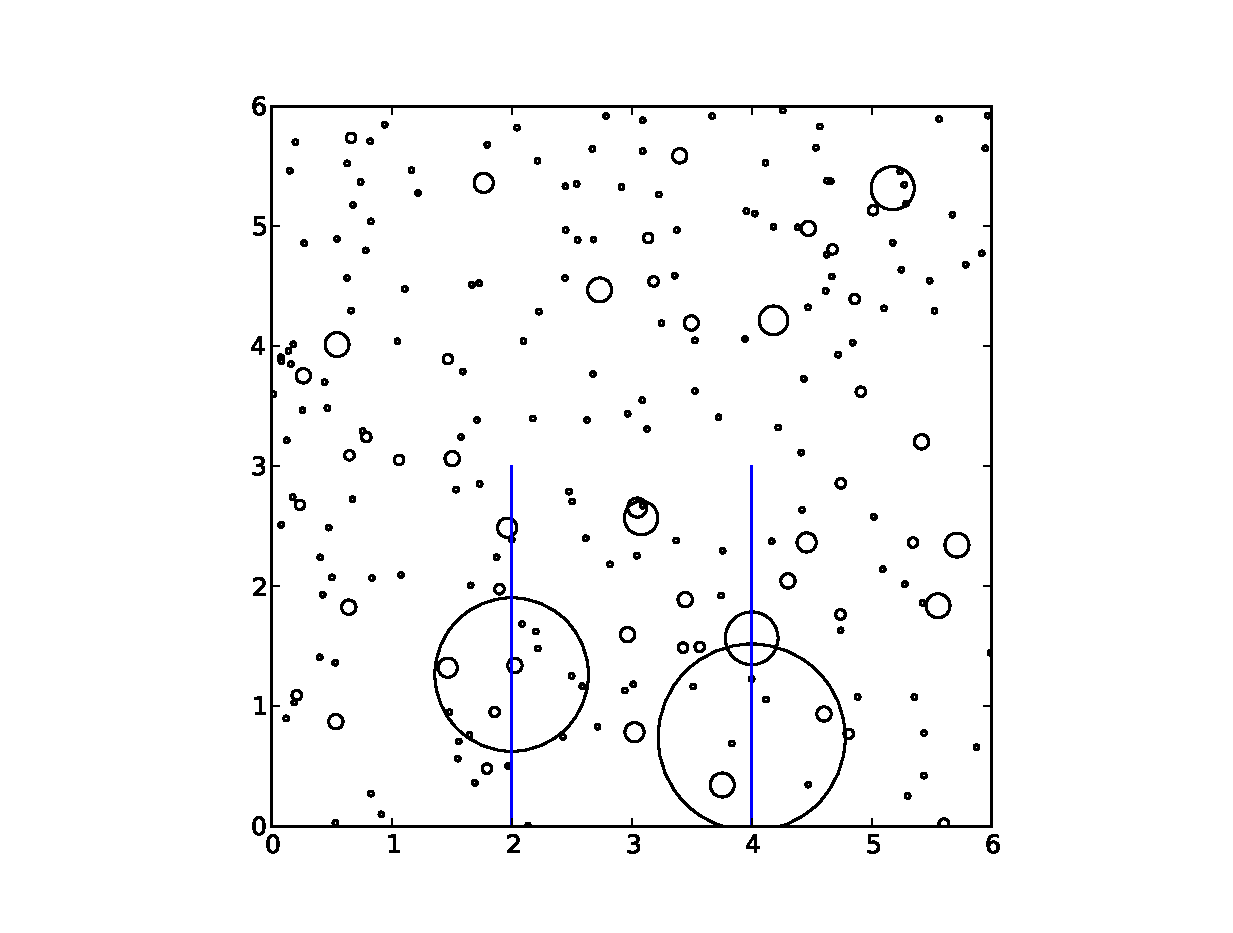
\includegraphics[width=\columnwidth]{../pics/1371544764.eps}}
\caption{В момент времени $t~=~600~\textup{с}$, вывод через pyplot}
\end{subfigure}
\caption{Внешний вид визуализатора.}
\end{figure}


	Микротрубочки в модели имеют вид вертикальных цилиндров с длиной, равной половине боковой стороны ограничивающего куба. В дальнейшем планируется усложнить модель, сделав более реалистичную структуру микротрубочек, например, представив их сеть в виде планарного графа. В таком случае, движение стрессовых гранул по ним будет возможно не только в одном направлении. При столкновении стрессовое гранулы с микротрубочкой они сцеплялись и в дальнейшем отсоединение не происходило, гранула начинала двигаться в одном из двух возможных направлений. Интересный вопрос, что делать при достаточно большом размере гранулы, когда она начинает касаться более одной микротрубочки. Согласно наблюдениям, гранула может двигаться вдоль любой из микротрубочек, что и объясняет сложность наблюдения за СГ в условиях запутанной сети. В данной модели считается, что переход от одной микротрубочки к другой невозможен.
	
	Случайное движение моделируется выбором шага по каждой оси координат согласно нормальному распределению со средним 0 и стандартным отклонением, зависящим от коэффициента диффузии следующим образом \cite{Michalet:2010uq}:
$$
	\overline{x^2} = 6Dt
$$
	
	Влияние микрофилламентов учитывается в пороге подвижности~--- считается, что при радиусе больше некоторого порога, гранула застревает в сети микрофилламентов и прекращает самостоятельное движение. В то же время движение возможно при движении микротрубочек~--- раз гранула не может оторваться от микротрубочки, она невольно будет двигаться вслед за ней.

	Была реализована платформа для проведение экспериментов. Для этого имеется возможность запуска серии симуляций с заданным набором меняющихся параметров. В системе предусмотрен вывод всех промежуточных результатов как на экран, так и в файл. Все результаты запусков сохраняются вместе с параметрами модели, при которых они были получены. Предусмотрен многократный запуск модели на одних и тех же входных данных для повышения статистической достоверности получаемых результатов. Система легко расширяема, внутри нее ведется журнал всех произошедших событий в хронологическом порядке для удобства анализа проведенной симуляции, на основе журнала возможен рассчет любых интересующих оценок.


\section{Результаты и обсуждение}
%Описания экспериментов, графики
\subsection{Частота столкновения между гранулами}
Исследуем время столкновения между стрессовыми гранулами при свободном блуждании без участия микротрубочек. Для это запускали моделирование со следующими параметрами:

\begin{itemize}
	\item размеры ограничивающего параллелепипеда: 6x6x6 мкм
	\item фрактальная размерность пространства: 1.8
	\item начальное количество частиц: 400
	\item количество микротрубочек: 0
	\item начальный радиус частиц: 20 нм
	\item порог неподвижности, начиная с которого стрессовые гранулы перестают перемещаться: 100 нм
\end{itemize}

\begin{figure}[htbp]\centering
\includegraphics[width=0.9\textwidth]{../results/P2pCollisionTimeOnDiffusionExperiment.pdf}
\caption{Зависимость времени столкновения между СГ от коэффициента диффузии.}
\label{fig:P2pCollisionTimeOnDiffusionExperiment}
\end{figure}

\begin{figure}[htbp]\centering
\includegraphics[width=0.9\textwidth]{../results/P2pCollisionTimeOnConcetrationExperiment.pdf}
\caption{Зависимость времени столкновения между СГ от их концентрации.}
\label{fig:P2pCollisionTimeOnConcetrationExperiment}
\end{figure}

Запускали при различных значениях коэффициента диффузии, для каждого значения запускали несколько (9) раз и брали значение медианы. Получили обратно пропорциональную зависимость (\autoref{fig:P2pCollisionTimeOnDiffusionExperiment}).

Теперь рассмотрим зависимость времени столкновения между гранулами от концентрации стрессовых гранул или же от их количества. Согласно теоретическим расчетам зависимость опять же должна быть обратно пропорциональной, что подтверждается моделированием (\autoref{fig:P2pCollisionTimeOnConcetrationExperiment}). Запускали при тех же параметрах, что и в предыдущем эксперименте.


\FloatBarrier
\subsection{Частота столкновения СГ с микротрубочками}
Проверим \autoref{eq:tm}, а именно зависимость среднего времени между столкновениями СГ с микротрубочками от длины и радиуса микротрубочек. Для проверки модель запускалась при переменной длине и радиусе микротрубочек соответственно и фиксированных остальных параметрах. Моделировались 300 секунд движения 400 гранул. Для чистоты эксперимента было отключено слияние стрессовых гранул при столкновении.

\begin{figure}[htbp]\centering
\includegraphics[width=0.9\columnwidth]{../results/P2mCollisionTimeOnLengthExperiment.pdf}
\caption{Зависимость времени столкновения СГ с микротрубочками от длины микротрубочек.}
\label{fig:P2mCollisionTimeOnLengthExperiment}
\end{figure}

\begin{figure}[htbp]\centering
\includegraphics[width=0.9\columnwidth]{../results/P2mCollisionTimeOnRadiusExperiment.pdf}
\caption{Зависимость времени столкновения СГ с микротрубочками от их радиуса.}
\label{fig:P2mCollisionTimeOnRadiusExperiment}
\end{figure}

\FloatBarrier
\subsection{Зависимость размера СГ от времени образования}
Проверим \autoref{eq:tg}, а именно зависимость времени образования гранулы определенного размера от ее радиуса. Моделировались 300 секунд движения 400 гранул. Для чистоты эксперимента было отключено слияние стрессовых гранул при столкновении.
Получили зависимость виду $y \sim x^{1.8}$, как и ожидалось.

\begin{figure}[htbp]\centering
\includegraphics[width=0.9\columnwidth]{../results/CreatingLargeGranulesExperiment.pdf}
\caption{Зависимость размера СГ от времени образования.}
\label{fig:P2mCollisionTimeOnRadiusExperiment}
\end{figure}


\FloatBarrier
\subsection{Зависимость времени столкновения между СГ от размеров клетки}
Рассмотрим зависимость времени столкновения между СГ от размеров клетки. Для этой зависимости нет теоретических формул. Результаты эксперимента говорят об обратно пропорциональной зависимости между величина, если число число гранул брать пропорциональным объему клетки, то есть третьей степени от размера боковой стороны.

\begin{figure}[htbp]\centering
\includegraphics[width=0.9\columnwidth]{../results/P2pCollisionTimeOnVolumeExperiment.pdf}
\caption{Зависимость времени между столкновения СГ от размера боковой стороны среды.}
\label{fig:P2pCollisionTimeOnVolumeExperiment}
\end{figure}


\section{Заключение}
Была реализована модель движения стрессовых гранул в среде в микротрубочками с броуновским движением частиц и взаимодействием с микротрубочками.

С помощью модели можно точно воспроизвести количество и размеры гранул, наблюдаемые \emph{in vivo}. Были поставлены эксперименты и получены параметры систем, отвечающих воздействию различных веществ на клетку.

Нами также были изучены зависимости между различными характеристиками, таким как время между столкновениями части и время образования гранул определенного размера и параметрами, такими как вязкость среды, концентрация инициаторных комплексов и прочими.

Полученные результаты согласовались с теоретическими выводами и позволили для формул с пропорциональностями получить точные коэффициенты.

Помимо этого, нами были изучены невстречающиеся в научной литературе зависимости между упомянутыми выше характеристиками и параметрами объема клетки и от размера ячейки актиновой сети.

Полученные закономерности позволят в лучшей степени изучить процесс образования стрессовых гранул в клетке и влияющие на него факторы.



\section{Выводы}
\begin{enumerate}
\item Были изучены стрессовые гранулы и роль микротрубочек в их движении.
\item Была построена математическая модель и реализована программа для симуляции и визуализации движения стрессовых гранул.
\item Были разработаны инструменты для проведения экспериментов и изучения зависимости модели от некоторого набора параметров.
\item На основе модели были проверены теоретические оценки: время столкновения между СГ от коэффициента диффузии и концентрации частиц, время столкновения между СГ на микротрубочках от длины и радиуса МТ и зависимость размера СГ от времени ее образования.
\item Были получены закономерности между временем столкновения между СГ от размера клетки и от размера ячейки актиновой сети.
\end{enumerate}

\clearpage
\nocite{*}
\bibliography{bibliography}



\section{Приложение 1. Исходный код}
%\lstinputlisting[label=sourcecode]{../src/sg_simulation.py}

\renewcommand{\theFancyVerbLine}{
  \sffamily\textcolor[rgb]{0.5,0.5,0.5}{\scriptsize\arabic{FancyVerbLine}}}


\inputminted[linenos,
             fontsize=\footnotesize,
%             framesep=2mm
             ]{python}{../src/sg_simulation.py}

\end{document}
